\chapter{Appendix A --- Expedition
Logistics}

\begin{quote}   
The majority of effort in organising an expedition is actually spent on the most mundane and domestic of matters.\\ 
\textbf{Jarvist Frost, Tarpaulins, May 21, 2011}
\end{quote}

One aspect that is often missing from expedition writeups is the
expedition logistics that enabled the exploration. For sure, this
information will be the fastest in this publication to age. For though the cave endures, and the human experience is understandable from year to year, technical progress makes a mockery of our carefully considered preparations.

    \begin{marginfigure}
\checkoddpage \ifoddpage \forcerectofloat \else \forceversofloat \fi
\centering
 \frame{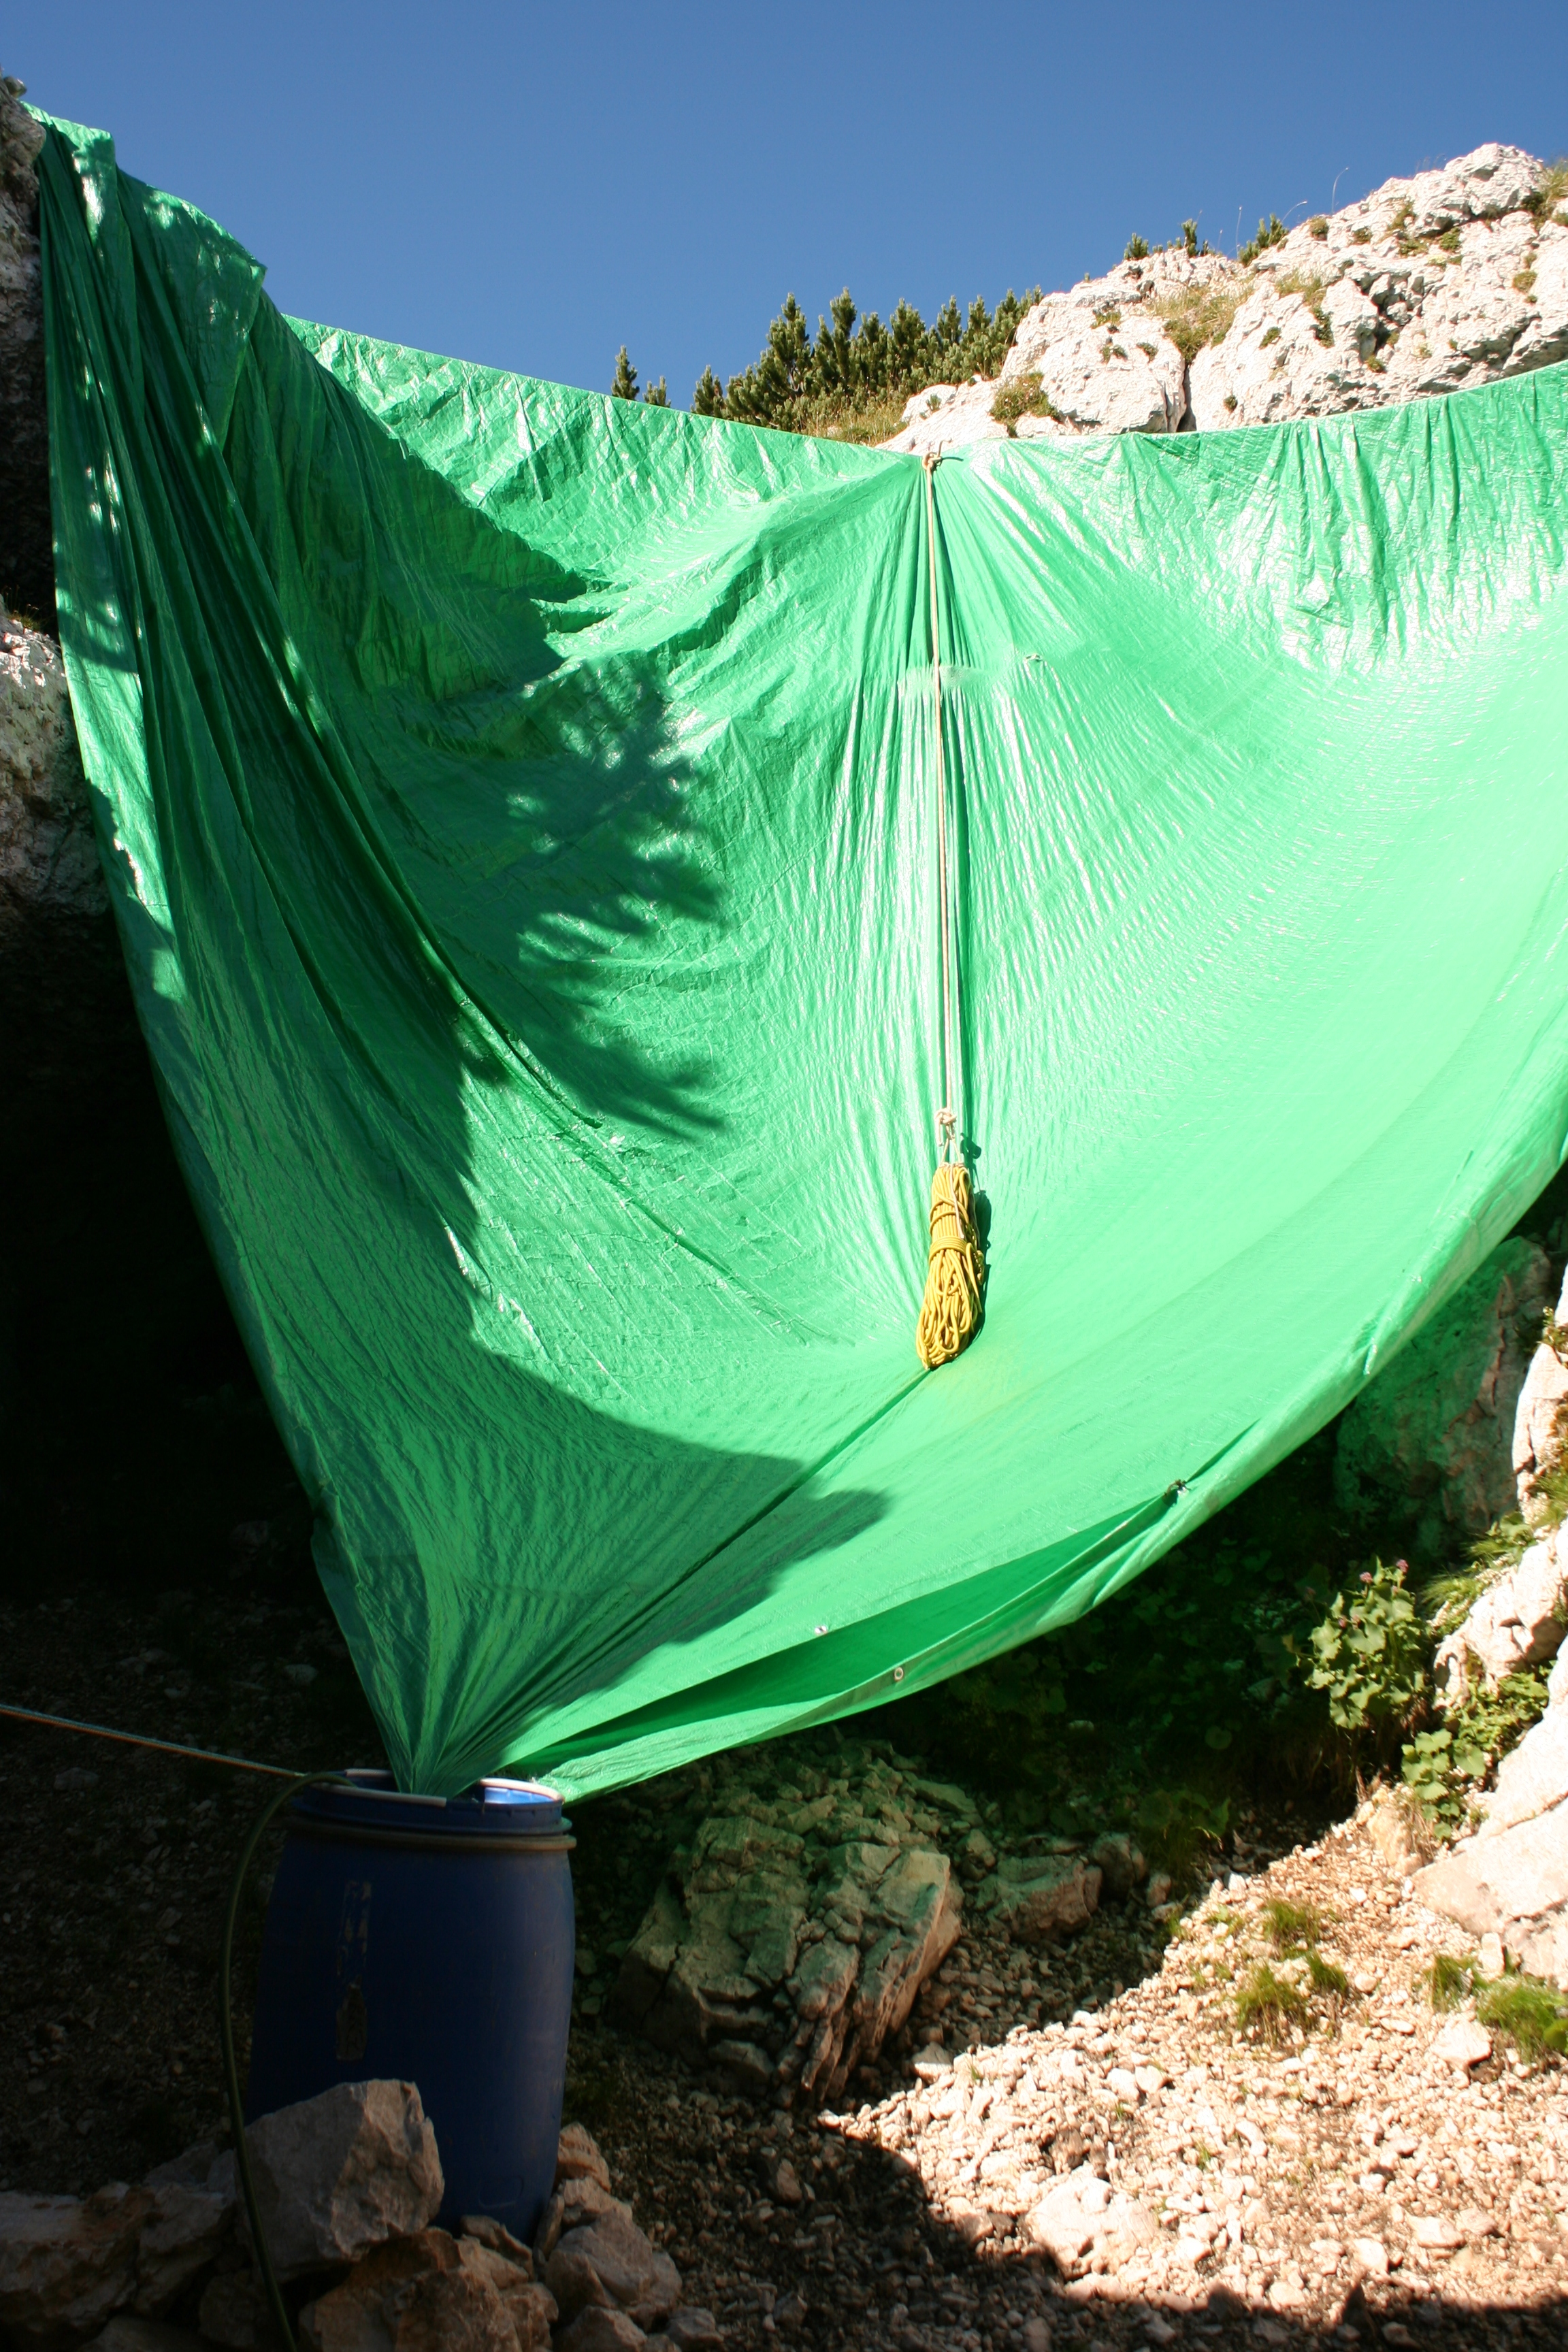
\includegraphics[width=\linewidth]{2010/ap_awards/20100801-07-58-16 - Jana Carga 06--orig.jpg}} 
 \caption{The tarpaulin in the back of the bivi known as the Sail. In 2010 it caught just as much air as water, and often tried to escape across the plateau. \pic{Jana Čarga}}
 \label{sail 2010}
\end{marginfigure}

During the period 2007--2012 covered here, we saw the total domination
of LED lights, displacing the previous carbide flames. Initially these
were mainly powered by Alkaline Flatpacks (helmet mounted) which gave
way to NiMh rechargeable packs as the brightness (and power input)
increased, and the length of our trips extended.

Our cave was rigged for Alpine style SRT, on Nylon rope. The main pitch
routes were rigged on 11 mm. Pushing was done on a mixture of 10 mm and
9 mm. Rope brands were selected for their toughness and ability to
resist abrasion more than ease of knot tying. Most of the caves were
rigged during this time on Mammut rope.

\begin{marginfigure}
\checkoddpage \ifoddpage \forcerectofloat \else \forceversofloat \fi
\centering
 \frame{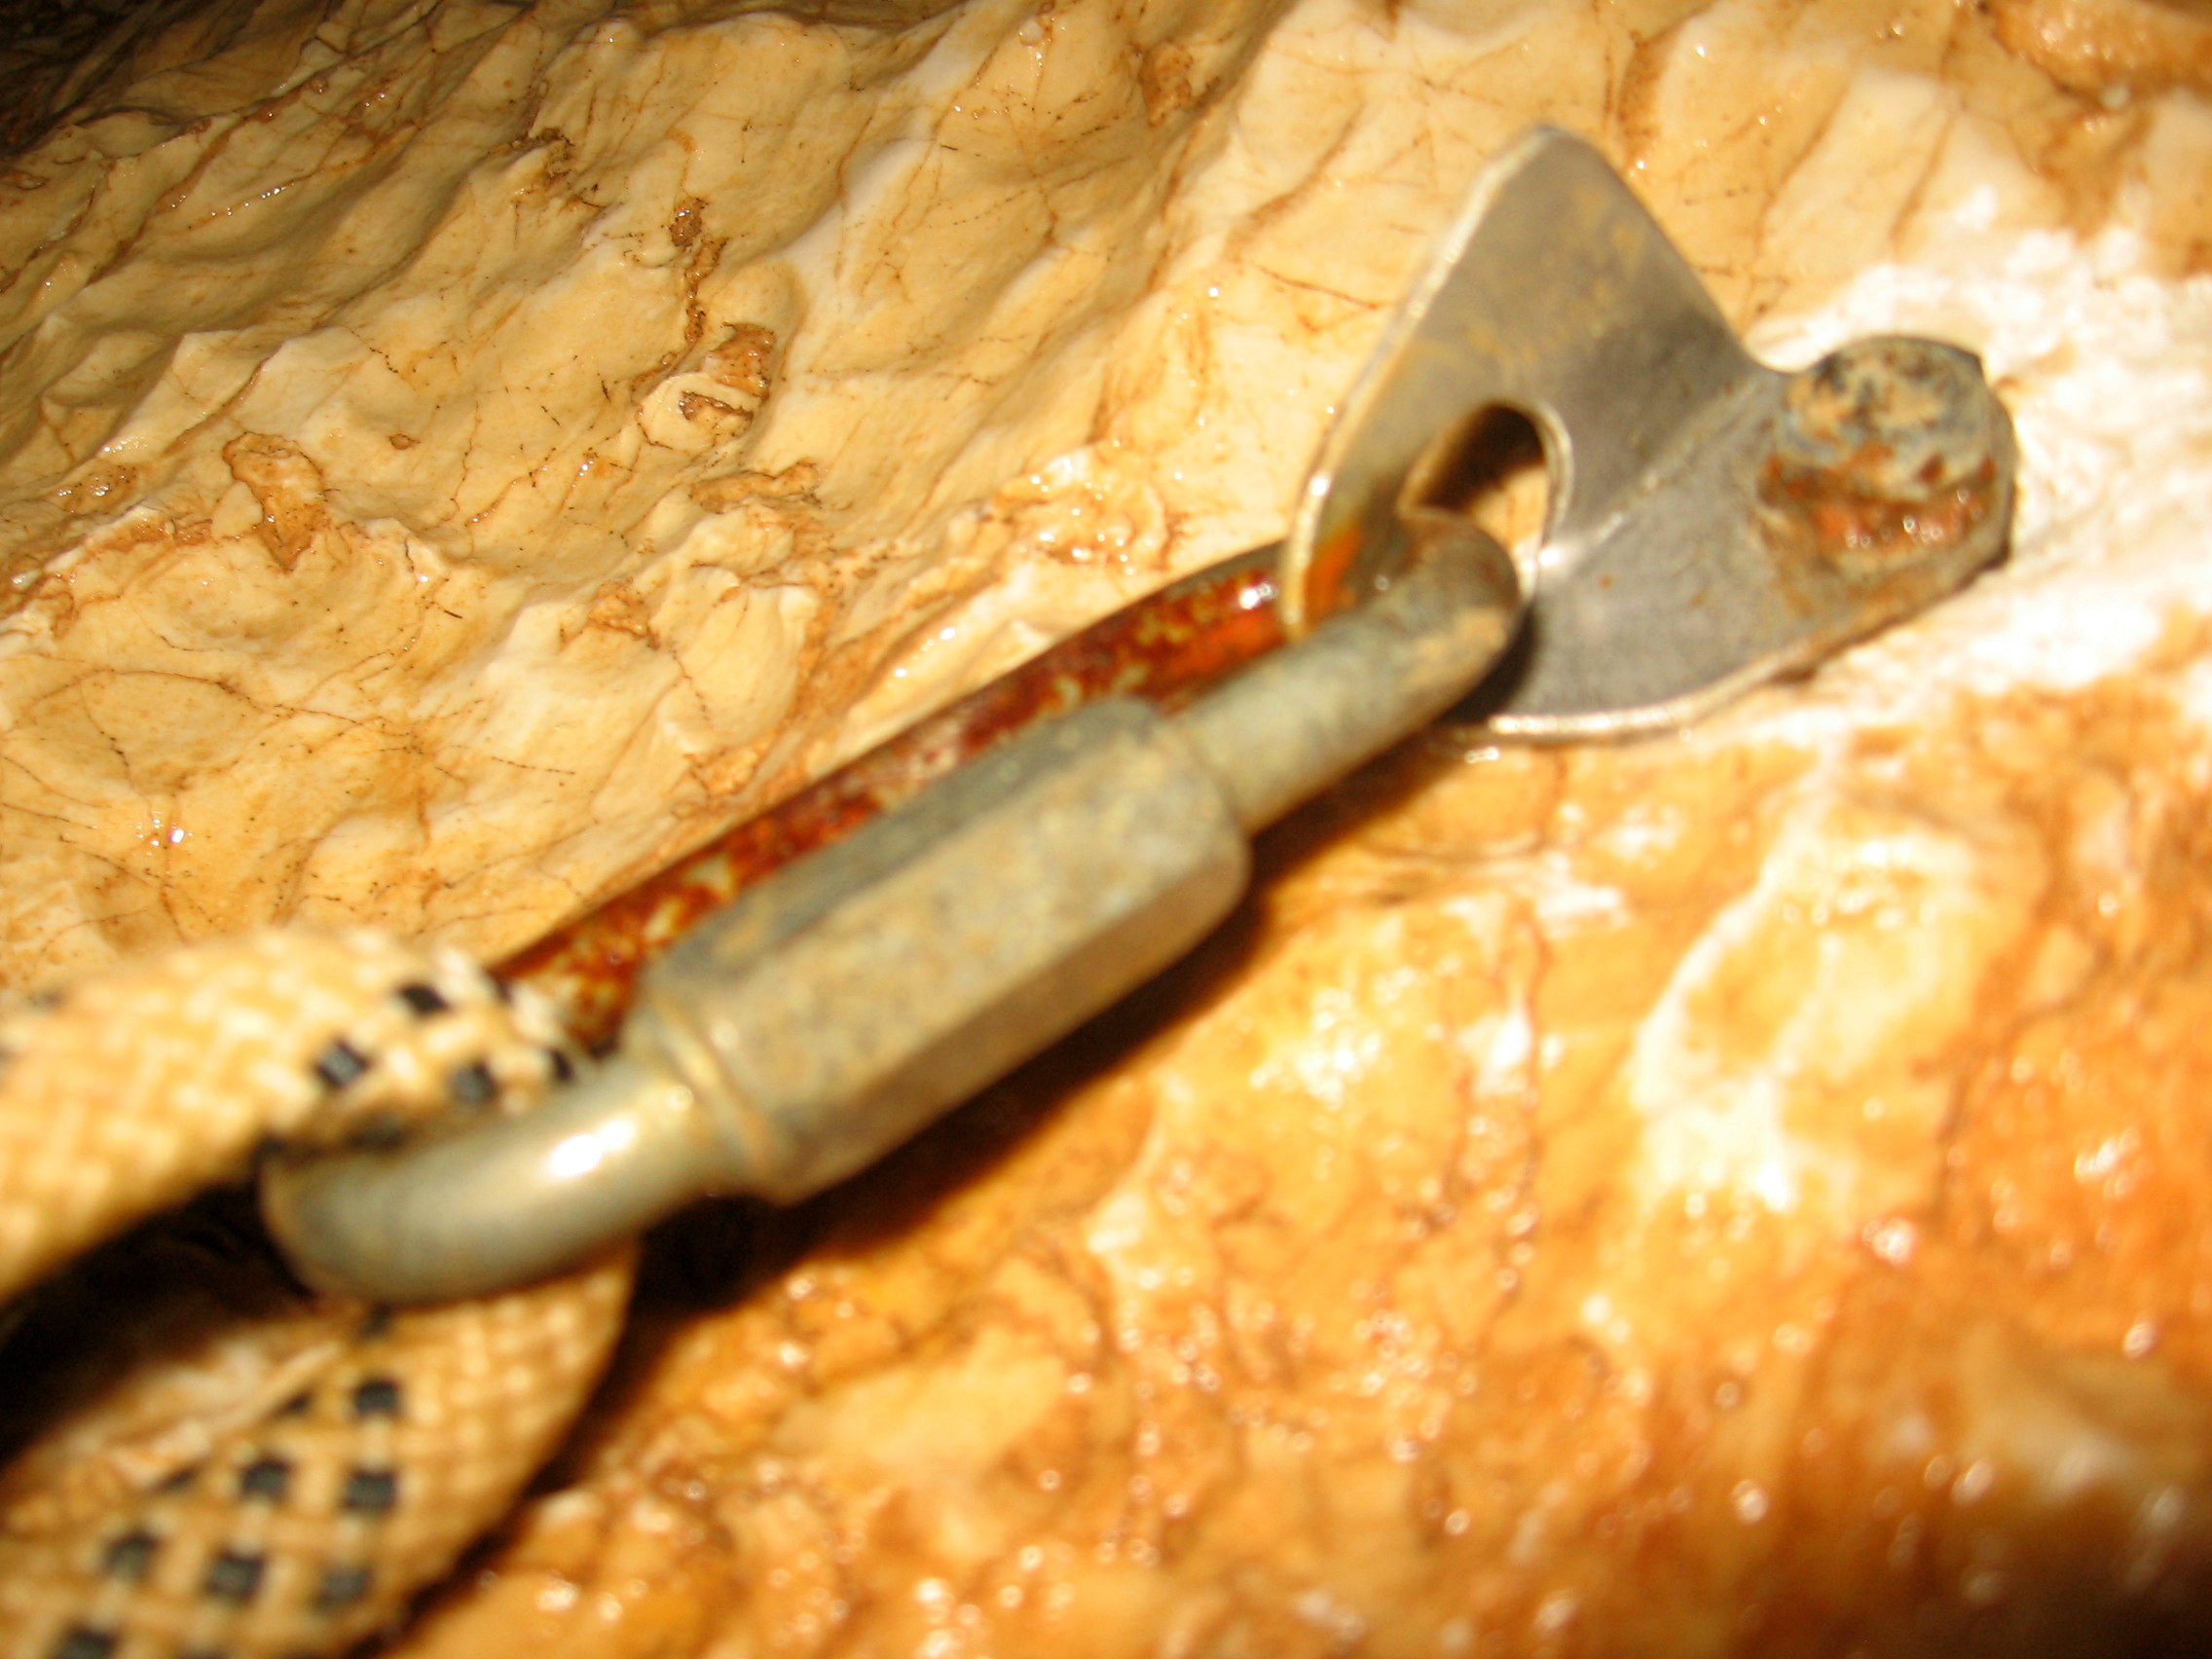
\includegraphics[width=\linewidth]{appendices/logistics/Jarvist Frost - canon a520 - sysmig - JC AJ trip - rusty maillon and homemade slov hanger--orig.jpg}} 
 \caption{Gone are the days of installing homemade hangers such as those shown here. \pic{Jana Čarga}}
 \label{homemade hanger}
\end{marginfigure}

The majority of bolting was with hand-bolted Spitz (mostly to Petzl
twist hangers), giving way in more recent years to 8 mm stainless through
bolts married with Raumer Stainless twist hangers. 7 mm long steel
maillons are used almost invariably for rigging.

There was approximately a 50:50 split with people wearing plastic
oversuits versus those of cordura. Most people caved with a normal
fleece furry and thermals, some stripping off for the prussic out.

\name{Jarvist Moore Frost}

\newpage


\section{Tarpaulins}
\textbf{\textit{May 21, 2011}}

Cave exploration gear is actually very simple to budget for—we have
a fairly good idea of how much rope we could possibly consume in a
given year of vertical development. You then need 1 bolt on average
per 10m of rope, and slightly fewer hangers / maillons (as you can rig
/ derig, scavenge, and some bolts will be failures). In a similar
vein, you need the same number of bolting kits and survey kits as
exploration teams you can realistically field, plus a few extras for breakages (particularly bolt drivers).

\begin{pagefigure}
      \checkoddpage \ifoddpage \forcerectofloat \else \forceversofloat \fi
      \centering
              \frame{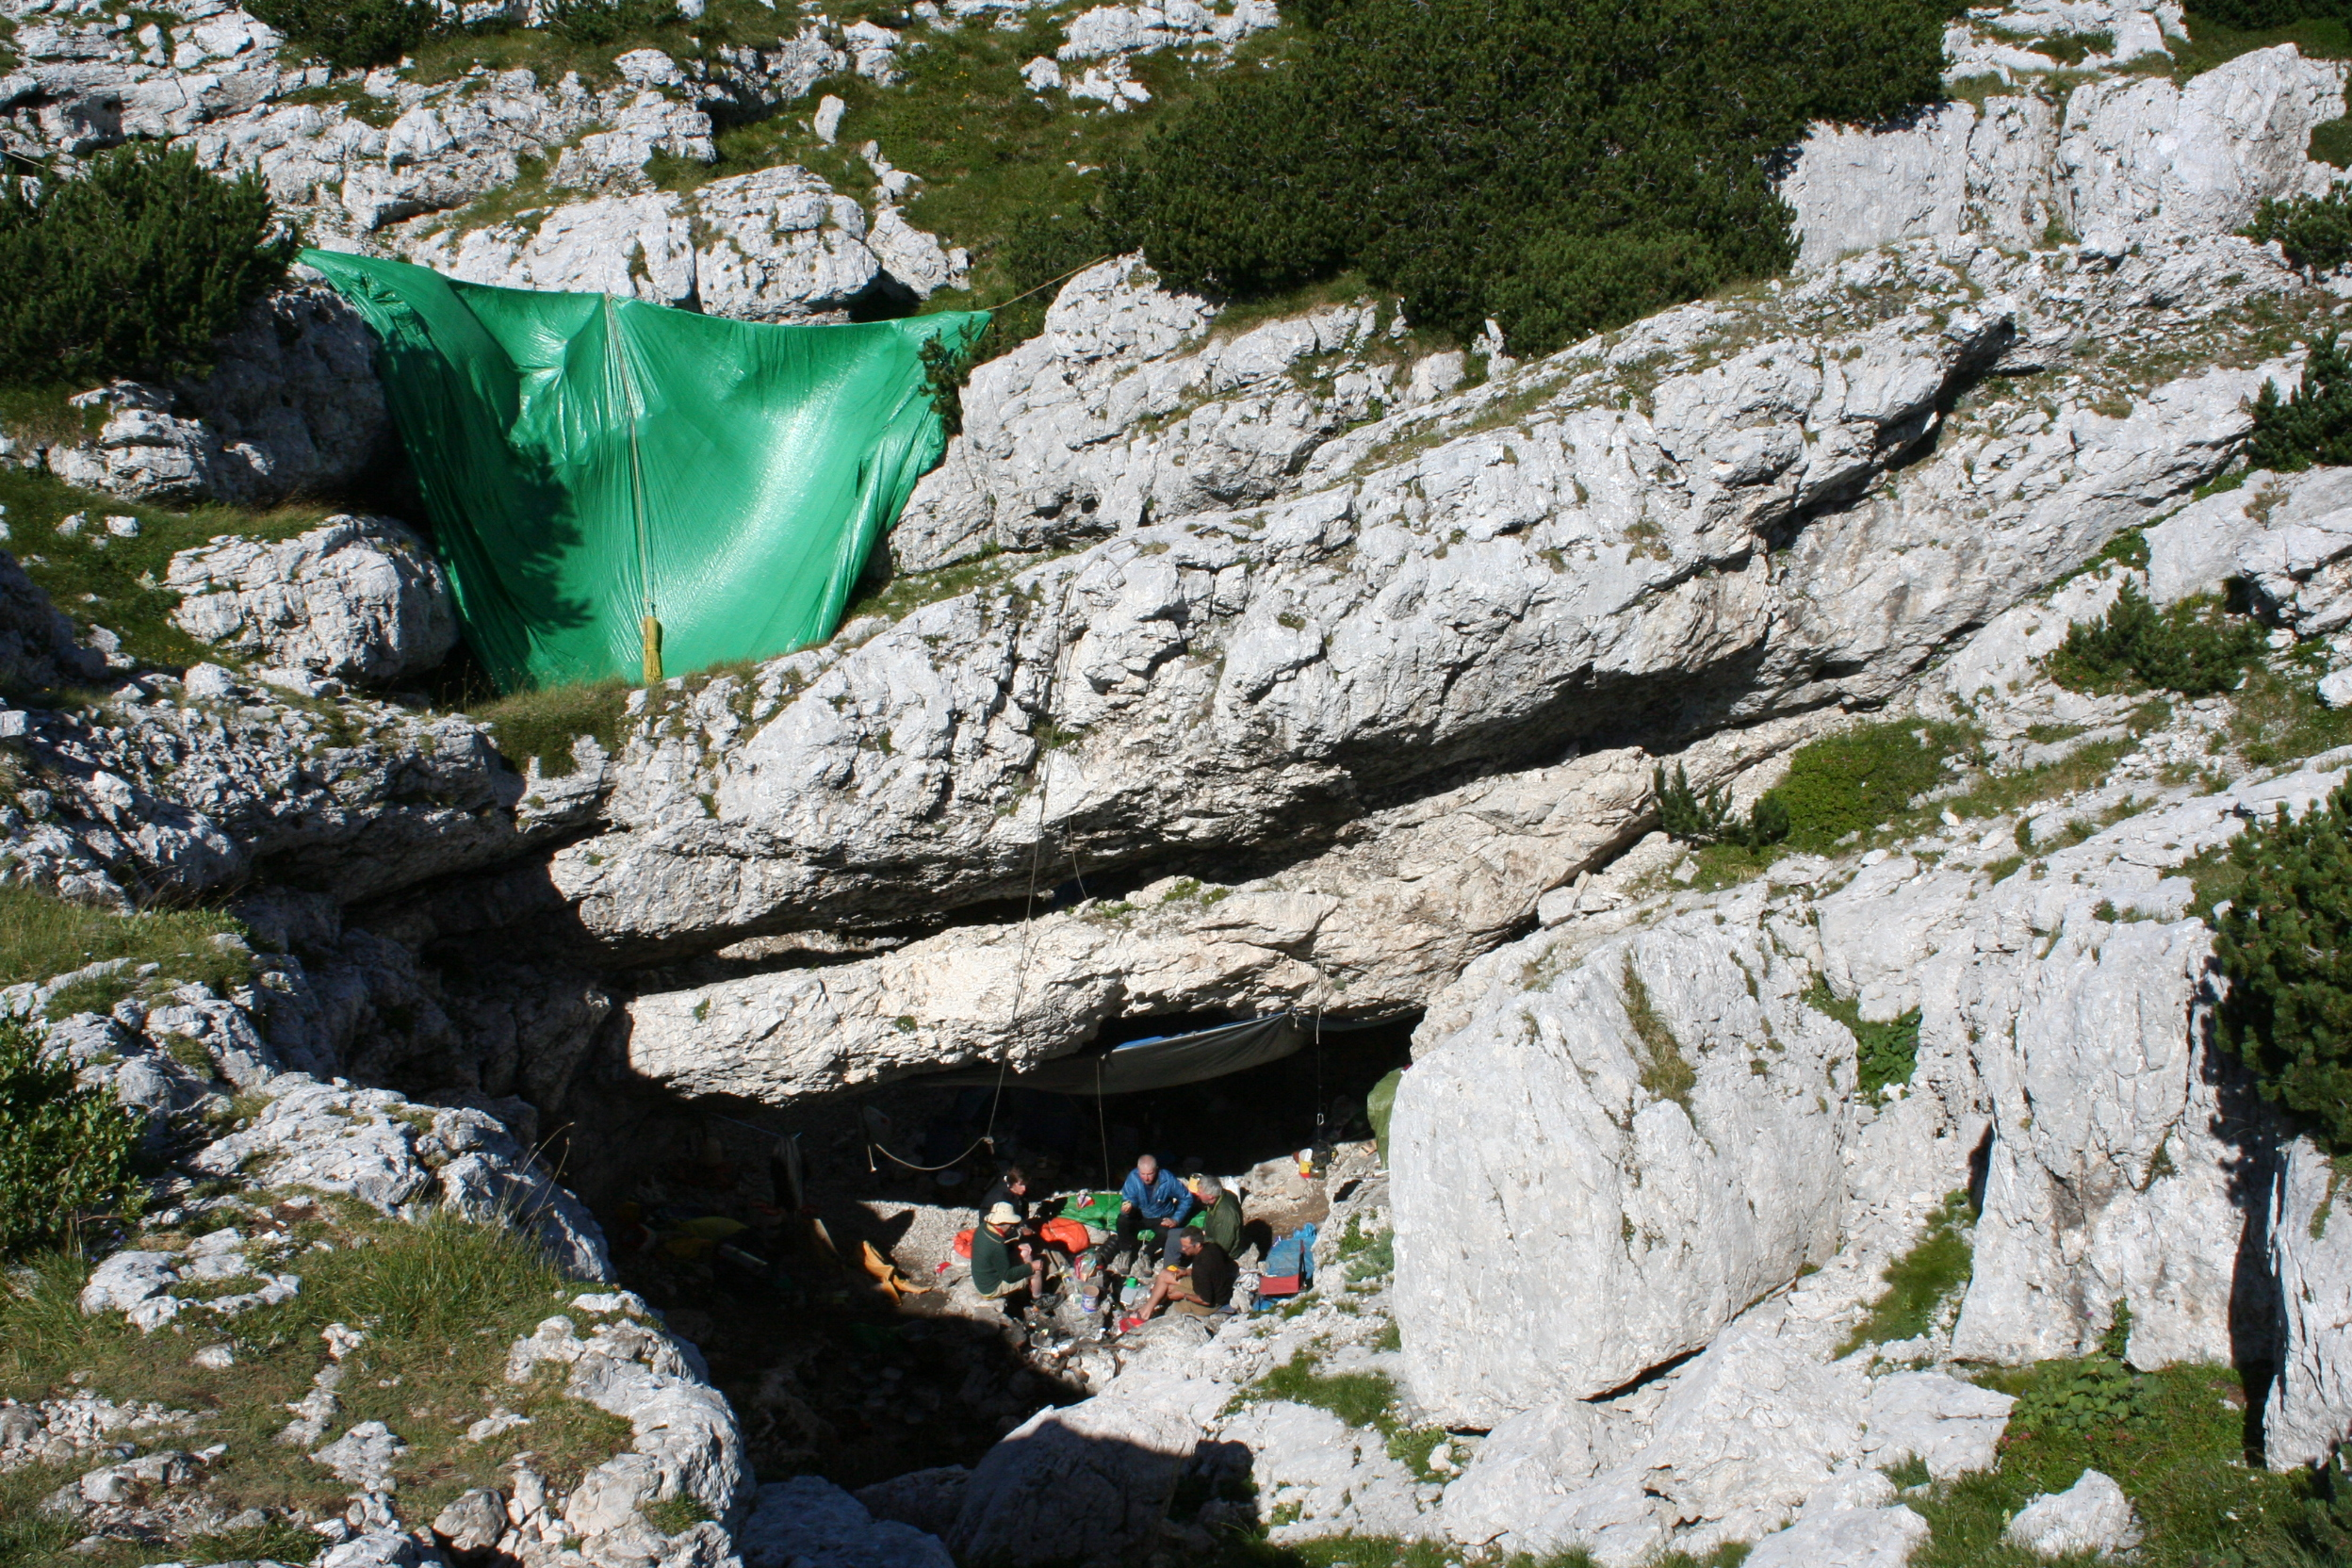
\includegraphics[width=\linewidth]{appendices/logistics/20100801-08-00-25 - Jana Carga 07--orig.jpg}} 
  \caption{The Sail is positioned in the back of the Bivi - an especially large one was extremely visible in 2010. \pic{Jarvist Frost}} \label{2010 big tarp}
\end{pagefigure}

We live in a shakehole with a rock bridge (Bivi). This is where all
the cooking takes place, food and caving gear is stored, preparations
are made for underground camp \& etc. Our water on top of the mountain
is mainly rainwater, collected into 200L blue barrels (which are used
during the winter to store dried food and equipment) off Tarpaulins
which also offer shelter from the rain for our gear and ourselves.

After much careful deliberation and consideration of photographs of
the Bivi, last year we bought a 9x14m Tarpaulin.
This turned out to be approximately twice as large as needed, and was
used doubled-up for the whole expo!


That massive green sail in the background of the photo is the Tarp—a
considerable amount of engineering went in to trying to prevent it
escaping across Skrbina! However, it did collect a vast quantity of
water when it rained.

So, 8 weeks before we set off again, we find ourselves with furrowed
brow in front of eBay, checking out the wares from a Tarp seller:
http://stores.ebay.co.uk/QVSonlineUK

The main tarpaulins we use for shelter are rather holey, and the brass
eye holes are mostly long gone (we find bunching the plastic and
tieing a choke knot to be more reliable anyway\ldots{}). Of course, we
intended to measure the current tarps properly with one of the many
tape measures we have out there, and draw a scale diagram of our
‘roof’, but it never quite happened\ldots{}

We’re definitely going with ‘heavy duty’ 170gsm tarpaulins this year,
but of what size? At 86–98 p/sqm, it’s something that you want to try
and get right first time! 

I’m currently thinking a 5.5M x 7M, 4M x 6M and a couple of small
tarps for general use\ldots{} £80 of the expo kitty on plastic sheeting
seems extravagant, but it’s nice to have drinking water \& shelter from
the storm!

\name{Jarvist Frost}



\section{Drills and Survey Instruments}


\subsection{Broken Uneo and New Suunto Instruments}
\textbf{\textit{June 18, 2011}}

\begin{figure*}
\checkoddpage \ifoddpage \forcerectofloat \else \forceversofloat \fi
\centering
    \begin{subfigure}[b]{0.49\textwidth}
        \centering
        \frame{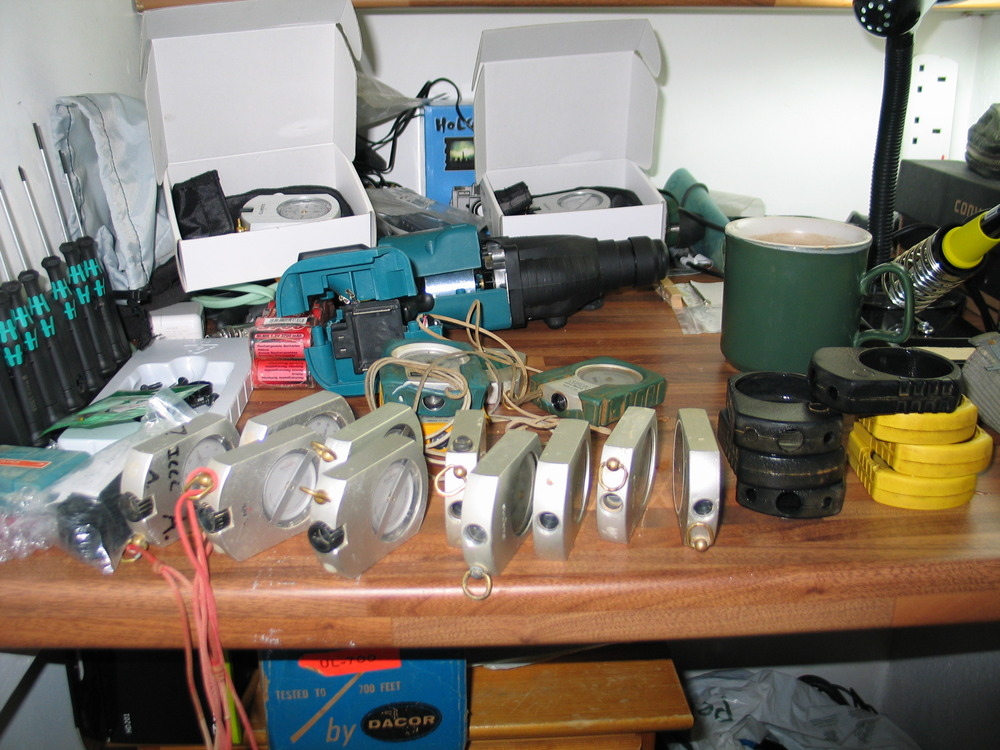
\includegraphics[width=\linewidth]{appendices/logistics/img_0007-scaled-1000.jpg}} 
        \caption{Survey instruments \pic {Jarvist Frost}} \label{survey instruments 2011}
    \end{subfigure}
        \hfill
\begin{subfigure}{0.49\textwidth}
\centering
\frame{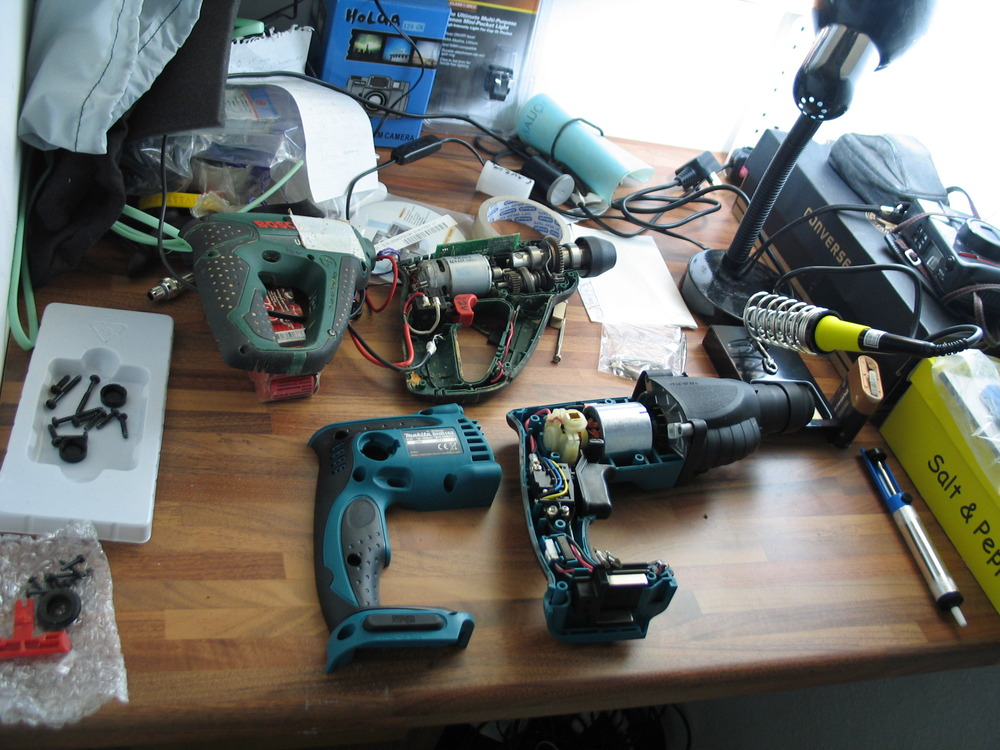
\includegraphics[width=\linewidth]{appendices/logistics/img_0005-scaled-1000.jpg}}
 \caption{Drills. \pic {Jarvist Frost}}\label{drills 2011}
\end{subfigure}
  \caption{}
\end{figure*}

The attempted bolt climbing practice in Yorkshire (May 2011) failed slightly with the death of the converted Uneo.

Drills — they promise so much yet deliver so little!

It’s a bit difficult to figure out what has happened to the Uneo. Certainly some chunk of the PCB seems electrically dead. The motor
works separately when wired directly to a battery, and the drill
electrics seem to flick on and off when there’s no motor wire in, but
in combination they’re dead! So it was off to eBay and within a few
days we’d acquired another new Uneo, this time for an even lower cost. So another drill to carefully take apart and solder in some
external leads\ldots{}

Our new set of Suunto survey instruments arrived courtesy of Wookey.
This was a good opportunity to fettle all the ones we presently owned,
so a good few hours were spent carefully wiping down the instruments
with a wet micro fibre cloth, removing cases, drying, opening the
diopter adjustments (on the >2006 instruments), carefully cleaning the
barrel and lenses, leaving to dry, reassembling, and finally attaching
the washed red necklaces and instrument covers. Phew.

A large proportion of the caving world has converted to swanky new
‘paperless’ surveying, with electric instruments \& bluetooth
connection to a PDA taken caving. Lots of different devices are
available, but perhaps the most popular is the DistoX [[
http://paperless.bheeb.ch/ ]]. If you go by what people talk about on
message boards on the internet, you may imagine that no one is left in
the world surveying on paper with manual instruments. I suspect this
is probably a publication bias; people who survey with computers like
talking about it on the internet, those with paper and pencil are just
getting on with it.

In my opinion, a big bonus of manual surveying in a ‘expedition’ based
cave exploration context is the egalitarian access to instruments —
they’re relatively cheap, last for years, and durable, so that every
team exploring can have a complete set rather than being the preserve
of an elite team or two. 

\name{Jarvist Frost}


\subsection{Makita BHR162}
\textbf{\textit{July 6, 2011}}

\begin{figure*}
\checkoddpage \ifoddpage \forcerectofloat \else \forceversofloat \fi
\centering
    \begin{subfigure}[b]{0.49\textwidth}
        \centering
        \frame{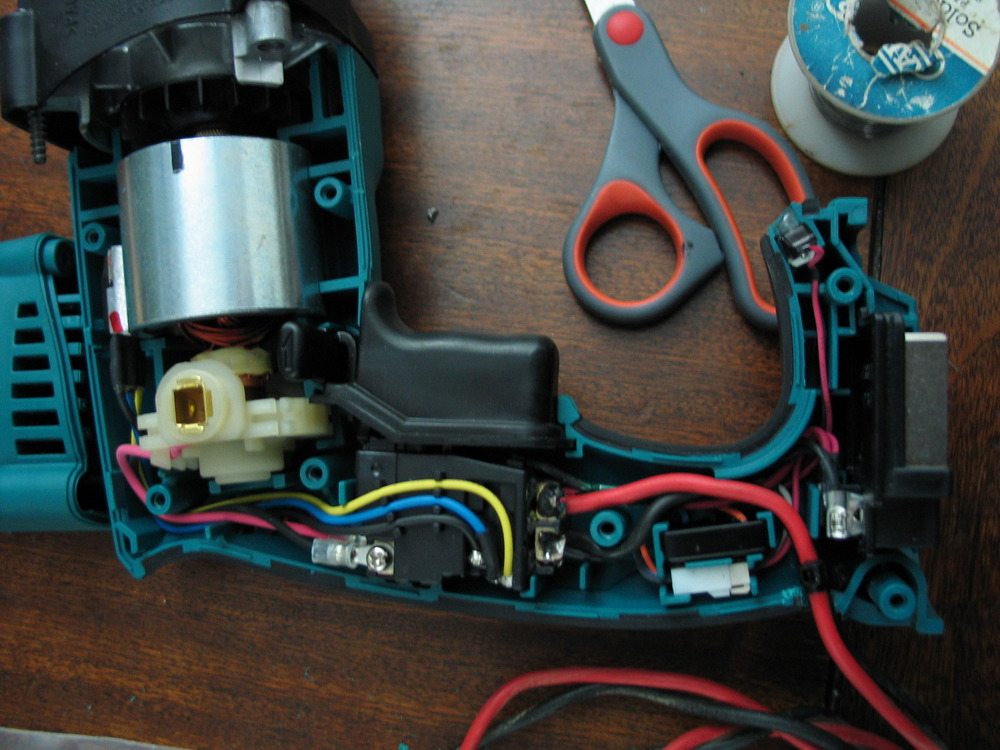
\includegraphics[width=\linewidth]{appendices/logistics/img_0087-scaled-1000.jpg}} 
        \caption{} \label{makita 1 2011}
    \end{subfigure}
        \hfill
\begin{subfigure}{0.49\textwidth}
\centering
\frame{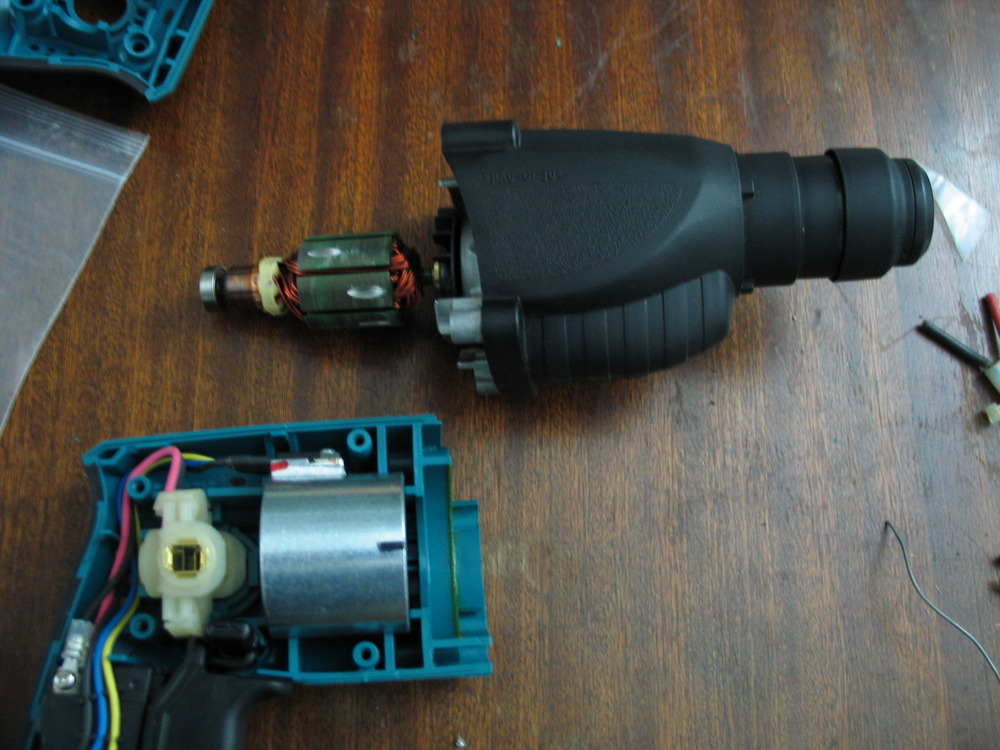
\includegraphics[width=\linewidth]{appendices/logistics/img_0088-scaled-1000.jpg}}
 \caption{}\label{makita 2 2011}
\end{subfigure}
  \caption{Attaching fly leads to the new Makita drill. \pic {Jarvist Frost}}
\end{figure*}


The Makita BHR162 seems a nice little caving drill, which happily runs
off 12V. There’s no funky electronics, just a variable speed control
and motor. The gear box assembly is in one piece, and there’s
environment seals over the switch and rubberised sections over the gap
between the two halves. Only issue is that it’s quite front heavy due
to the dense gearbox, perhaps not the best drill for bolt climbing
(Uneo!) but a nice lightweight SDS-plus for general use and abuse.

The designers even left two spare screw holes on the variable power
trigger to add fly leads for an external battery, without needing to
disable the normal external.

Having taken it apart a few times, my recommended disassembly is something like:

\begin{itemize}
    \item Set to non-hammer to lock pneumatic mechanism
    \item Remove carbon brushes
    \item Unscrew 4 long screws that hold gearbox onto body of drill
    \item Pull stator / motor out of enclosure by pulling on gearbox assembly (you might want to get a flat blade screwdriver in the gap between gearbox back (metal) and body so you don’t start pulling the gearbox to pieces. The motor will be fairly stiffly stuck by the permanent magnets).
    \item Unscrew all the little screws in the body
    \item Split apart body
    \item Have your wicked way with a soldering iron
    \item Reverse to reassemble!
\end{itemize}

\name{Jarvist Frost}



\newpage

\section{Three Years at X-Ray: Underground Camp Logistics}

\begin{marginfigure}
\checkoddpage \ifoddpage \forcerectofloat \else \forceversofloat \fi
\centering
 \frame{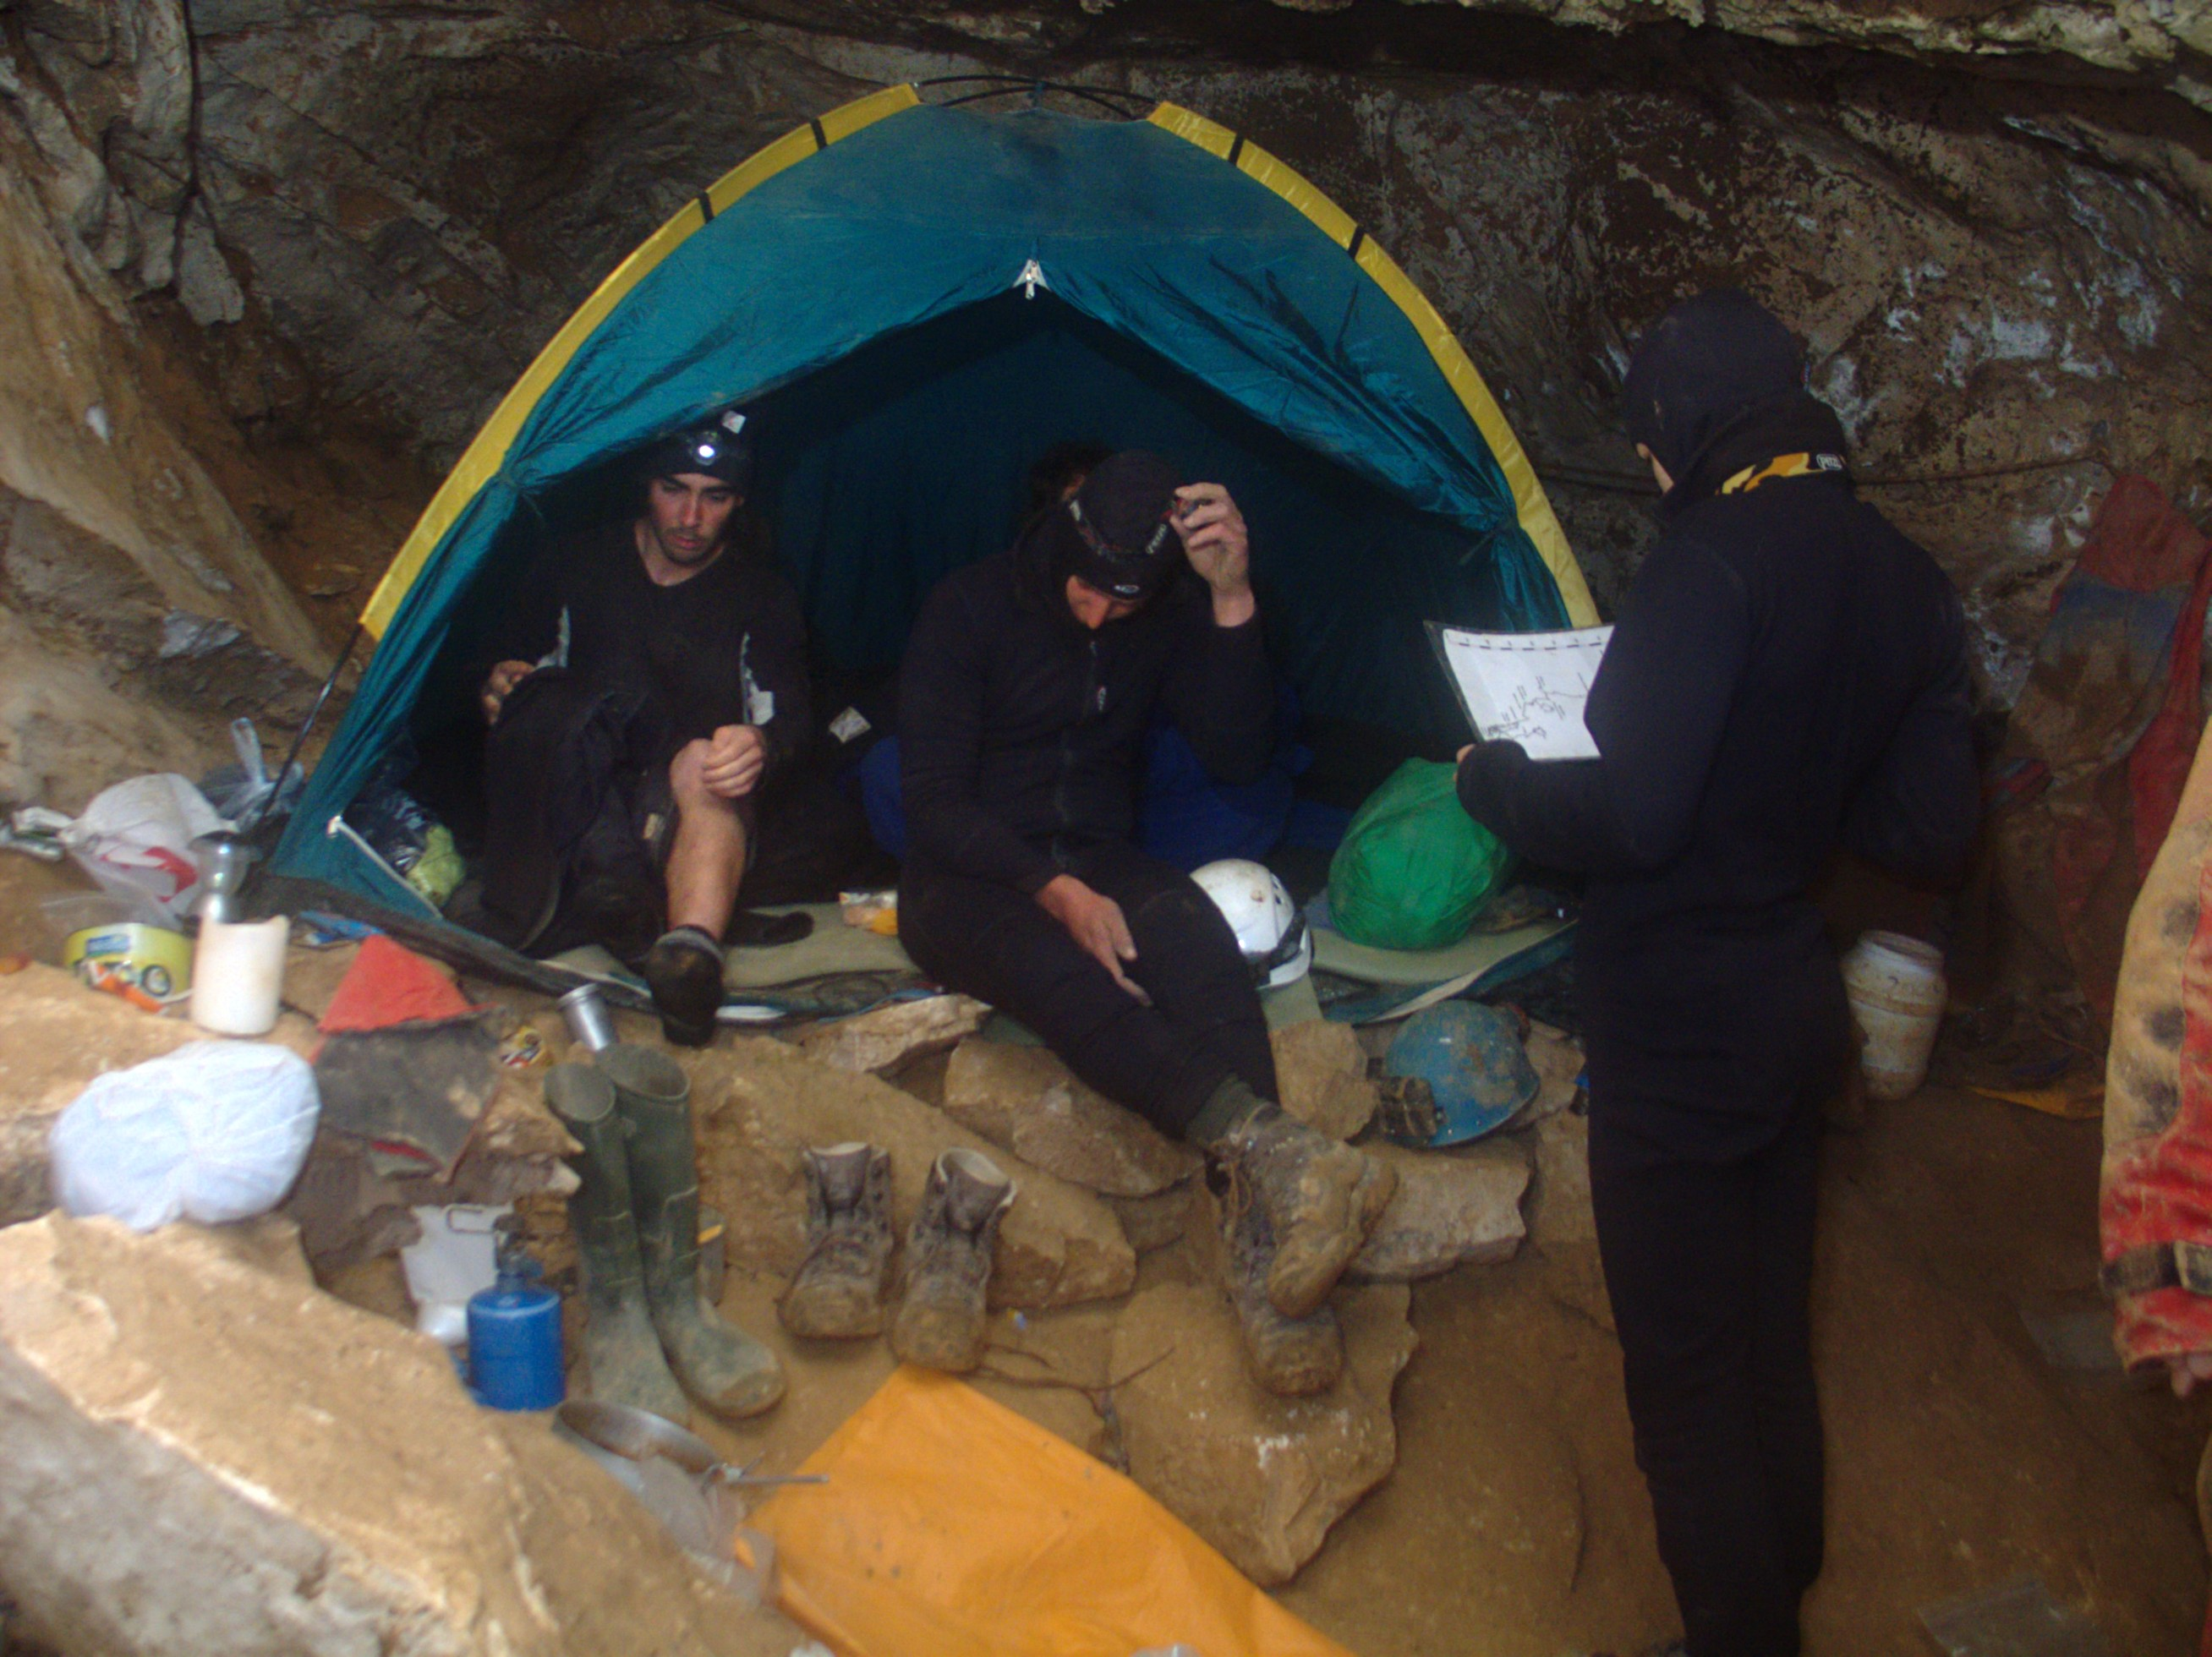
\includegraphics[width=\linewidth]{appendices/logistics/20100802-09-10-10-Jarvist Frost-Canon G5-CRW_0471-Camp X-ray--orig.jpg}} 
 \caption{Camp \protect\passage{X-Ray}. \pic{Jarvist Frost}}
 \label{camp}
\end{marginfigure}

The Vodna Sled 2010 4-berth underground camp was extremely comfortable
and provided an excellent base for extended deep cave exploration.

As there seems to be little information written about setting up alpine
caving camps, we describe in this document an overview of the equipments
used, and resulting performance. This camp was used almost unaltered in
2011 and 2012, and we have included a few updates and tweaks gained
during those expeditions.


\section{Cave Conditions}

\passage{Vrtnarija} is a typical deep alpine cave system. The temperature measured at camp varies between 2 and 5 degrees centigrade.

Camp \passage{X-Ray} has a fairly considerably draft which flows from the (wet) \passage{Zimmer} pitch. We would estimate the relatively humidity to be above 80\%, and note
that non-sealed paper becomes damp overnight.

\section{Sleeping Arrangements}

\subsection{Tent}

An extremely cheap 4-person single-layer dome tent was purchased from eBay. The tent fabric was washed at 60°C in a large washing machine with an excess of detergent in order to remove the water repellent coating and thus reduce condensation. This appeared to have been entirely successful -- no beading was apparent.

The tent notably increased temperature and comfort at camp.

It was found impossible to close the doors fully due to the feet of
anyone above about 1.6m poking out the foot of the tent, but having the
bottom zip open was found to produce suitable airflow.


\subsection{Sleeping Bags}

\begin{marginfigure}
\checkoddpage \ifoddpage \forcerectofloat \else \forceversofloat \fi
\centering
 \frame{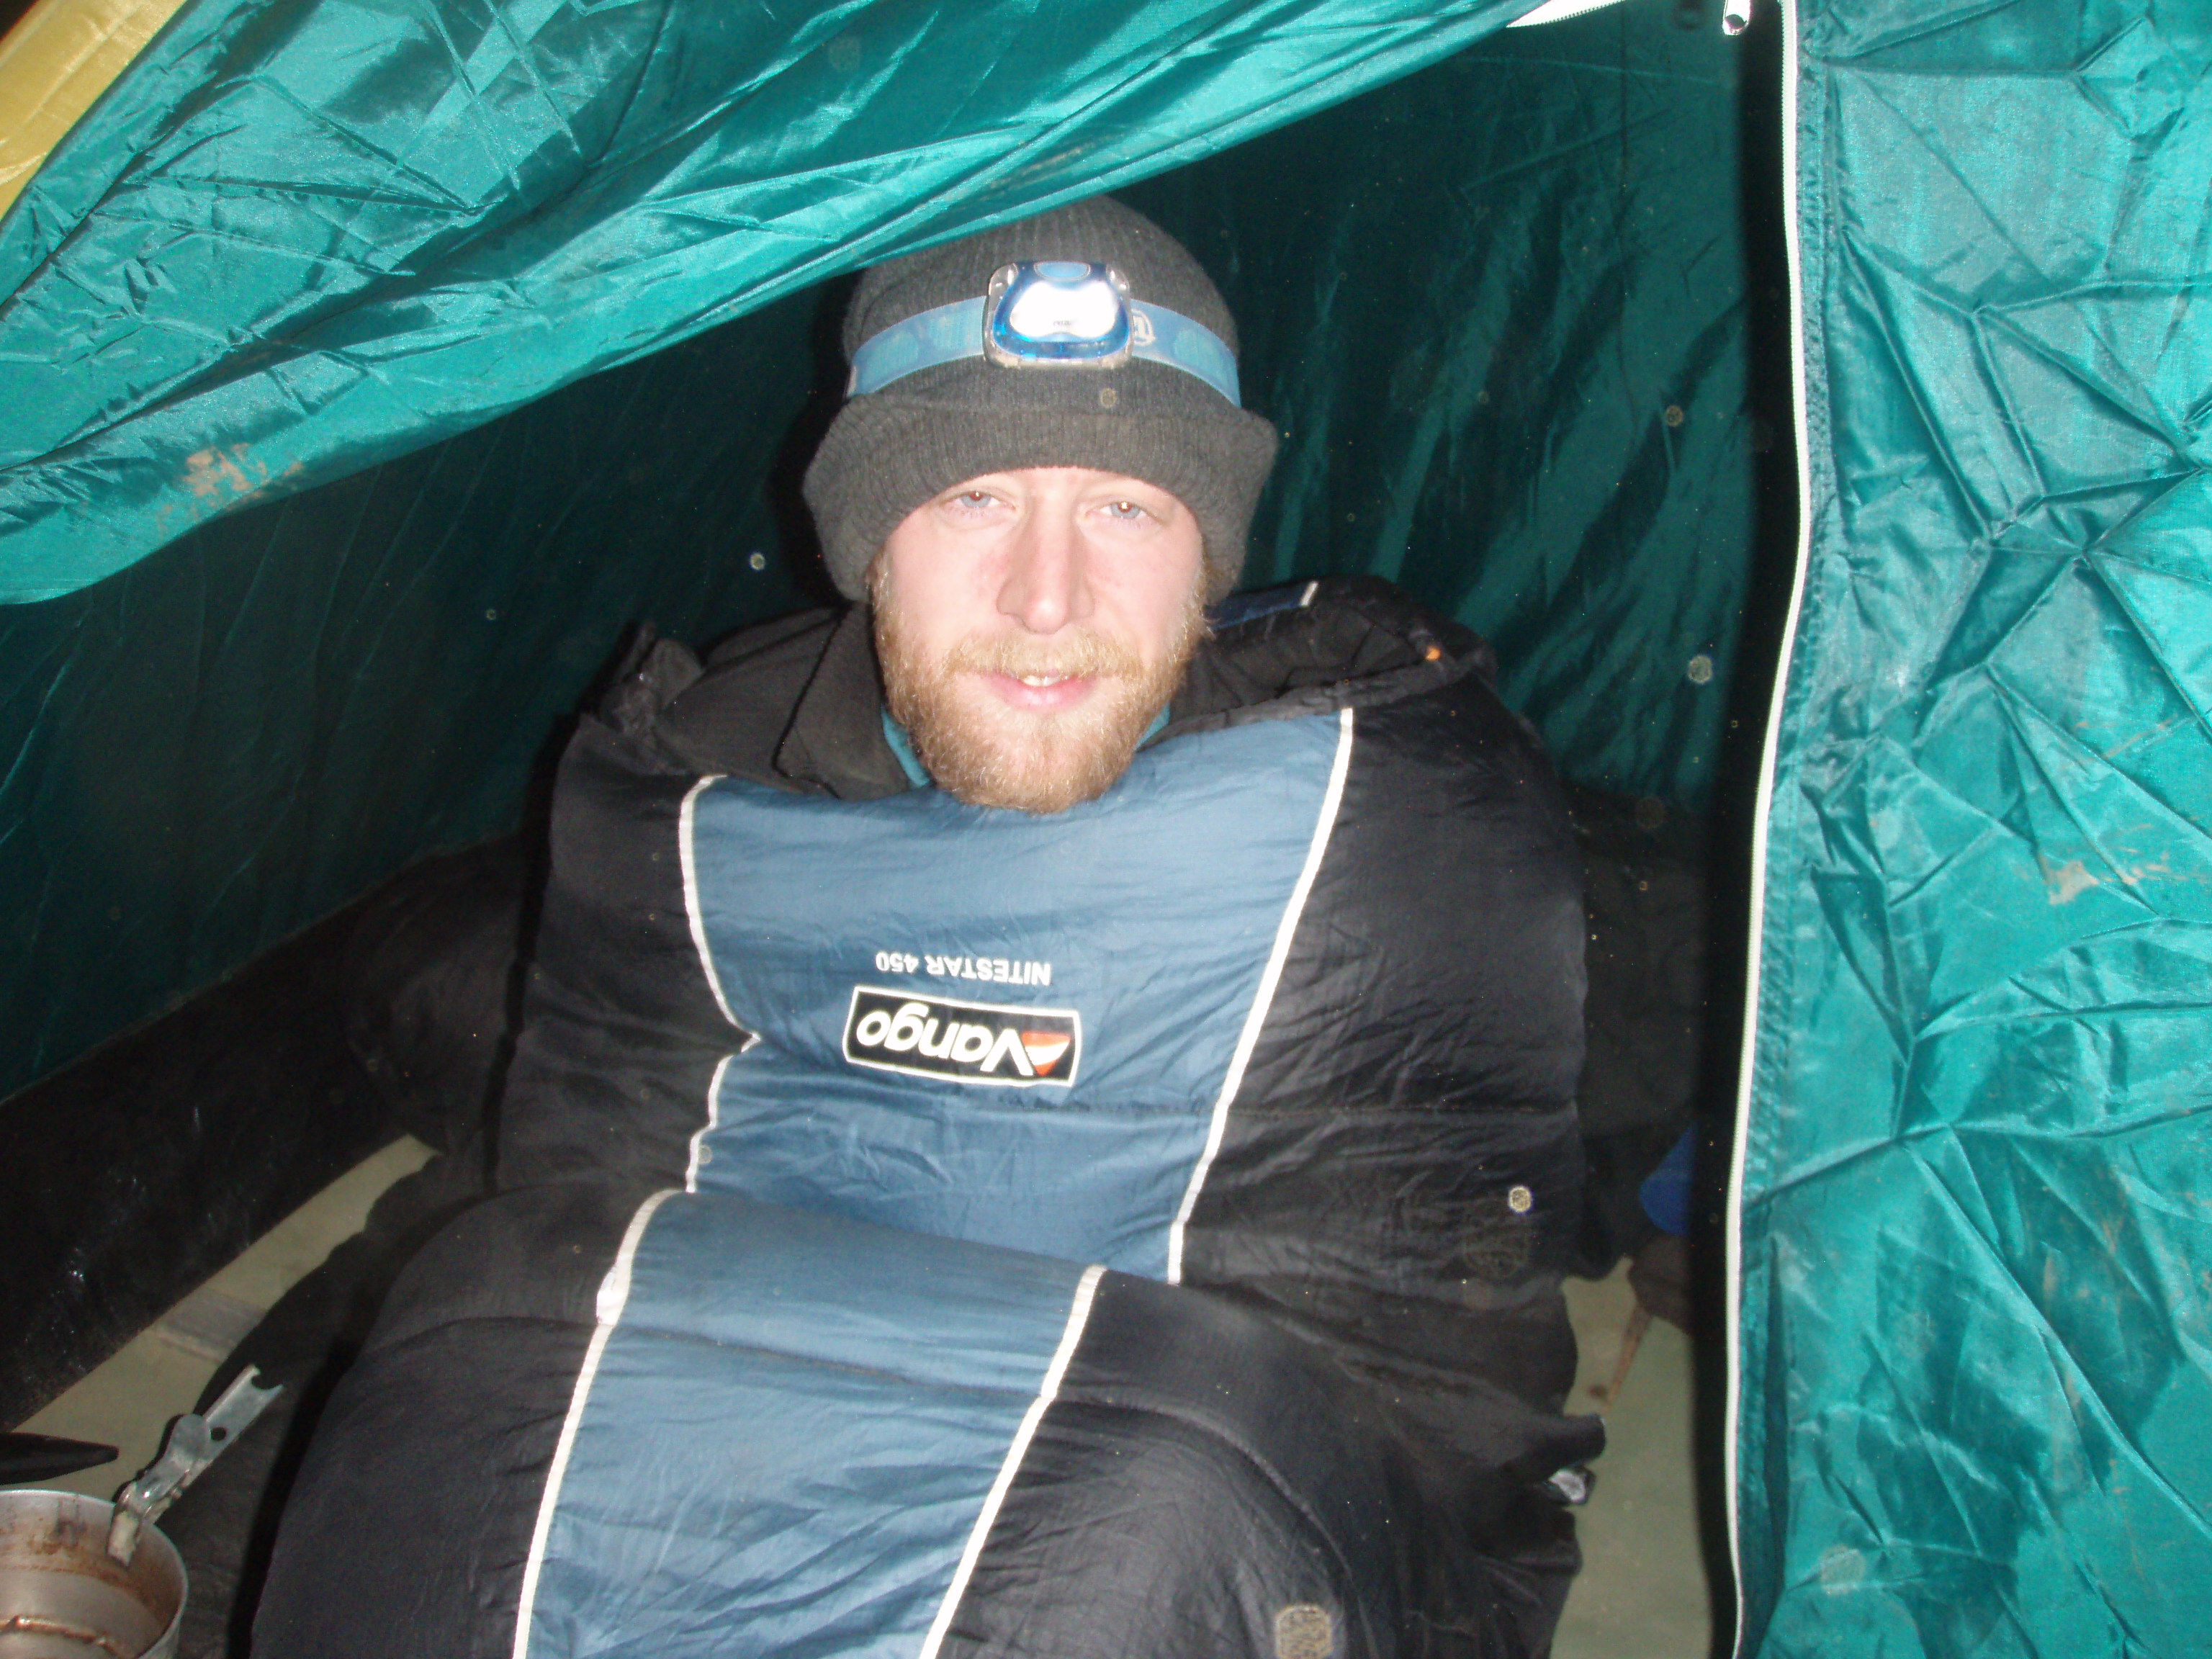
\includegraphics[width=\linewidth]{appendices/logistics/20100807-20-30-49 - Jan Evetts - P2070111 - Camp X-ray--orig.jpg}} 
 \caption{Jan Evetts inside a Vango Nitestar 450 at camp \protect\passage{X-Ray} in 2010. \pic{James Kirkpatrick}}
 \label{nitestar 450}
\end{marginfigure}

In 2010 two of our berths were 1990s Buffalo bag fibre-pile liners, supplemented with 200g sqm polartec fleece liners (supplied a long long time ago as sponsorship in kind).

In these, most campers also required the wearing of a full set of fleece thermals within these bags to remain suitably warm (Beast Sponsorship in 2009).

It was also difficult to actually get within the multiple layers of sleeping bag, and one found oneself rather constrained once there.

By comparison, two of the beds were made out of Nitestar 450 synthetic bags, purchased for $\approx$ £30 each. These were found to be warm enough on their own, though small women in particular had a more comfortable night when wearing fleece pyjamas.

A suggestion for future underground camps is to add synthetic silk (nylon) liners to further increase the warmth.

The bags weigh 2kg each, but are extremely bulky. Packing the bags back in London, we were able to fit the sleeping bag and fleece pyjamas in one large oval tackle sac. For the derig, we only managed to pack the sleeping bag alone into the same large tackle sacks.

We replaced the Buffalo bags with more Nitestar 450 sleeping bags in 2011. The later 2011 edition Nitestar 450s are entirely synthetic (no cotton in the liners) and thus almost the perfect underground camp sleeping bag. They feel noticeably less damp and sticky on the skin when you first get in them.


\subsection{Roll Mats}

We now use `Nato 5 season' roll mats produced by Highlander / Outdoors value for circa. £10. They are long enough for the 2m tall folk.

Colour: Olive green, Size: Open: 180 x 50 x 1cm, Rolled size: 50 x 15cm, Weight: 300g

Superb compression recovery, Density: 25kg/CBM.


\subsection{Condensation}

Condensation was minimum except for underneath the rollmats, as is common for camping in cold conditions, and a slight temporary damping of the top of the rollmat underneath the sleeping bag head.

One thing that was avoided was the careless use of superfluous fleece camp clothes as a pillow -- it was found that this material provided a wick for condensation.


\section{Cooking Arrangements}

\begin{marginfigure}
\checkoddpage \ifoddpage \forcerectofloat \else \forceversofloat \fi
\centering
 \frame{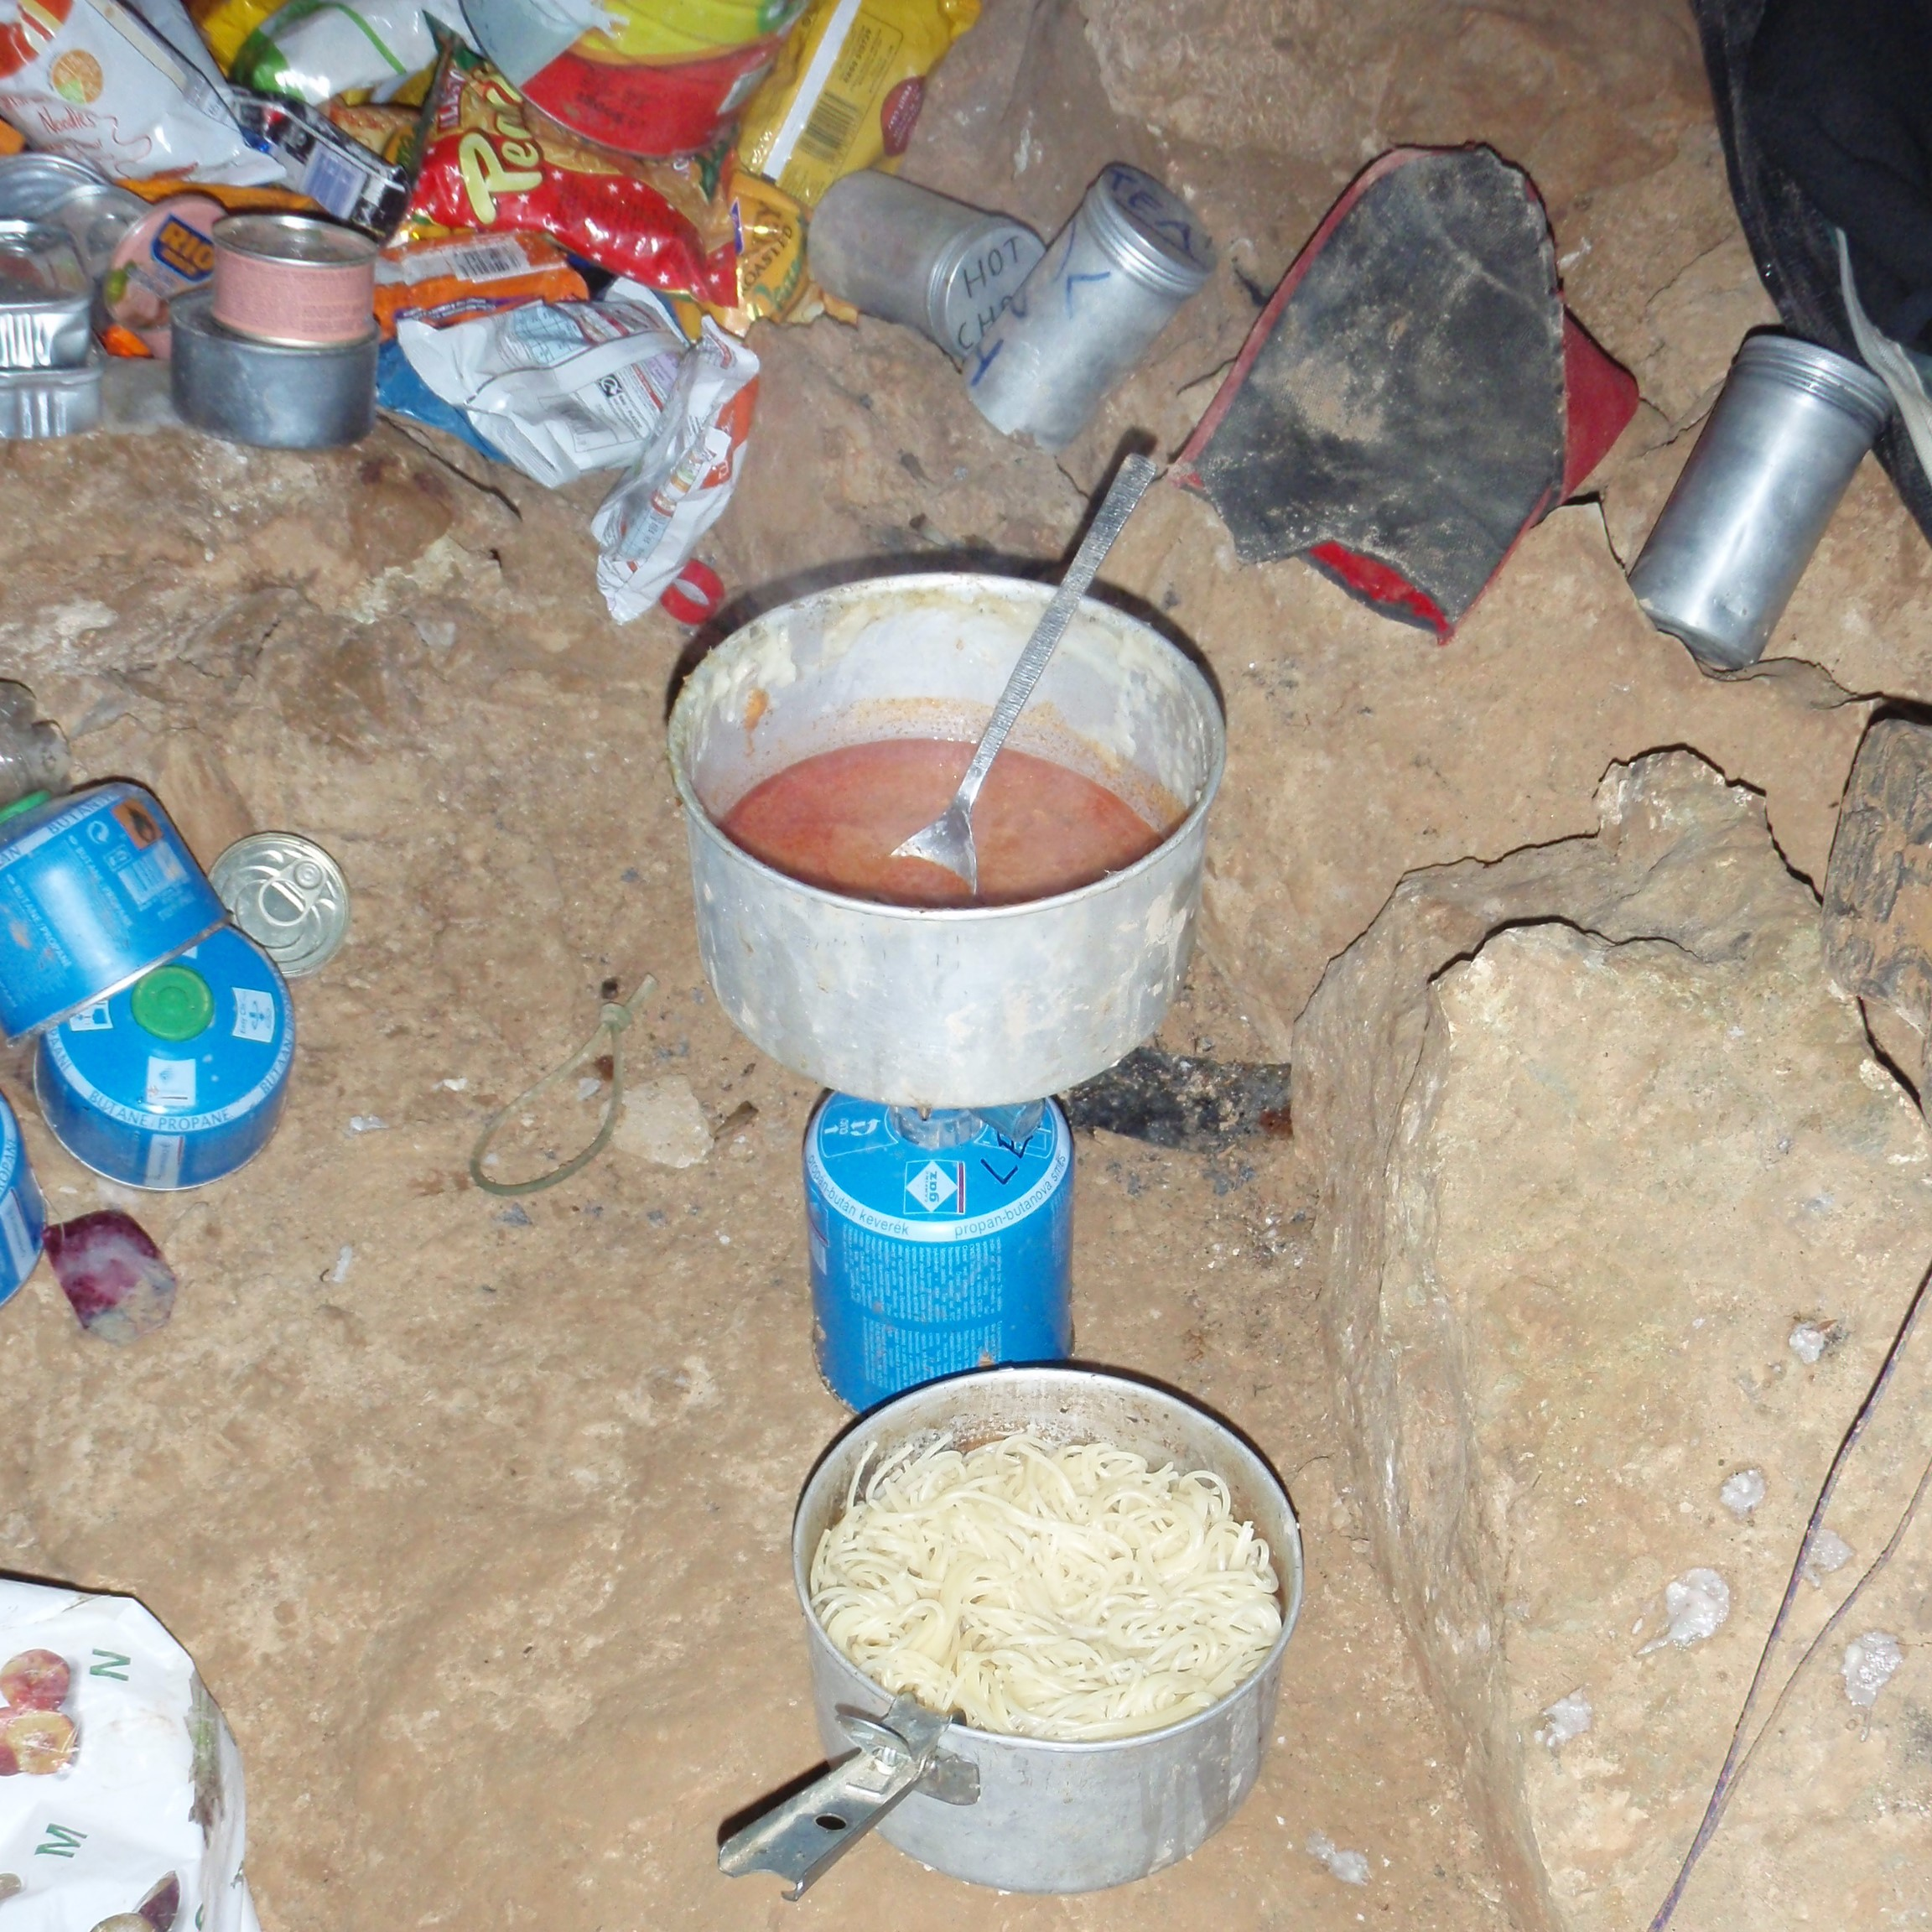
\includegraphics[width=\linewidth]{appendices/logistics/20100802-12-33-30 - Iztok Mozir - P8024766 - Camp X-ray--square.jpg}} 
 \caption{A typical meal cooked at underground camp: soup and noodles. \pic{Iztok Možir}}
 \label{soup noodles}
\end{marginfigure}

Cooking at underground camp consisted of a Mini Trangia; recycled MSR aluminium windshield for the Trangia; Campingaz Micro Plus Gas Stove; `SunnCamp Trekker 5 Piece' Aluminium nesting cook pots (17cm and 18cm sizes, including the 19cm lid / frying pan); clasping pot handle; 4 `lightmyfire' nylon sporks.

All this was packed into the largest 18cm saucepan and weighed circa \textasciitilde{}1.5kg.

In general the trangia burner was used with the largest saucepan to cook the breakfast / supper meals and was found to be sufficient for 4 people.

The medium saucepan was kept clean (ish) to be used to make hot drinks.

The small trangia saucepan was used to make small drinks (for instance herbal tea / coffee when others were drinking black tea), and for particularly dietry requirements (vegan) or simply to hold cut up cheese / salami during preparation.

In 2011 the `Campingaz' stove was replaced with a cheap `universal screw fitting' then used with Primus Powergaz 4-season gas mix (we noticed we were ending up with a frozen slurry of unburnt gas in our normal summer mixes).

This new gas setup is really quite powerful, perfect for a quick hot drinks.

Usually drinks are made as soon as cavers return / wake, drunk while still undressing, with the food more slowly cooked on the Tranja.


\section{Food \& Drink}

Fish, Cheese, Soup and Smash were the general, standard permutations.

However, there was also significant quantities of instant noodles (Sainsbury / ASDA own brand), CousCous (in particular the Ainsley Harriet branded flavoured variety) and even Risotto mixes.

Other cooking ingredients included dried mushrooms and dried tomatoes, vegetable bouillon mix, miso soup mix and sesame seeds.

\begin{marginfigure}
\checkoddpage \ifoddpage \forcerectofloat \else \forceversofloat \fi
\centering
 \frame{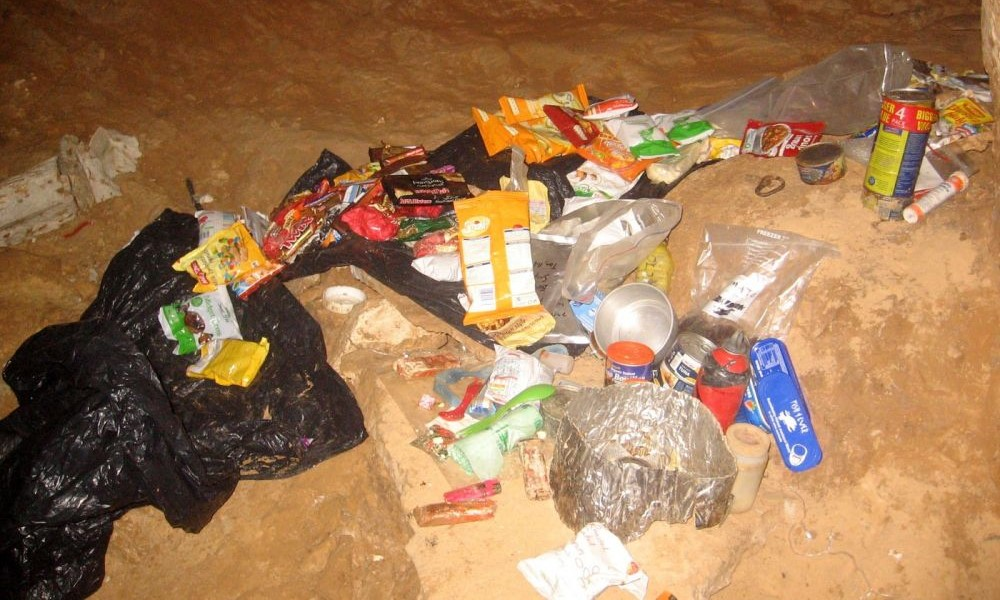
\includegraphics[width=\linewidth]{appendices/logistics/2011-08-01-13.24.46-Jarvist M Frost-CanonA520-IMG_0175 - Food Reserves and Stove at Camp X-Ray--orig_1050p.jpg}} 
 \caption{Food reserves at camp. \pic{Jarvist Frost}}
 \label{food reserves}
\end{marginfigure}

Condiments included smoked paprika and black pepper which had been freshly ground on the surface and transported underground in a 35mm film canister.

`White Powders' and other such bulk ingredients were taken down in ultra-strong resealable plastic bags (100micron -- bought from `thermalpaper' a dedicated plastic bag ebay.co.uk reseller), with the contents written on in clear black marker pen.

Drinks, almost always warm or hot, were based on black tea (Yorkshire Tea), local herbal teas (in particular Sadni Chi), hot chocolate (Makro own brand) and Vitaminski (an effervescent flavoured vitamin drink actually called `Cedevita').

Lunches were generally the standard caving snack food (chocolate bars, midget gems, peanuts -- in particular honey roasted from Lidl), but also supplemented with oatcakes and bread with salami, cheese and fish.

Spirits were taken down in 500ml plastic bottles and used as a small nightcap by the majority of cavers.

The rolling hot-bed camp meant that every 12 hours all underground cavers were physically present at camp, and therefore had their callouts reset on a rolling basis.


\subsection{Saving Fuel \& other camp
craft}

A considerable number of tricks and tips were taught by the seasoned expeditioneers to save on fuel and increase enjoyment at underground camp. All simple, but useful, ideas.

\begin{itemize}
\item
  Smash doesn't need boiling water to make.
\item
  Noodles require boiling water, but can be cooked in a small volume of
  water, then have cold water added along with Smash to thicken.
\item
  Tea can be more efficiently made by boiling half the required volume,
  making strong tea, then mixing 50:50 with cold water to make an
  immediately consumable drink.
\end{itemize}


\section{Music \& Entertainment}


\begin{marginfigure}
\checkoddpage \ifoddpage \forcerectofloat \else \forceversofloat \fi
\centering
 \frame{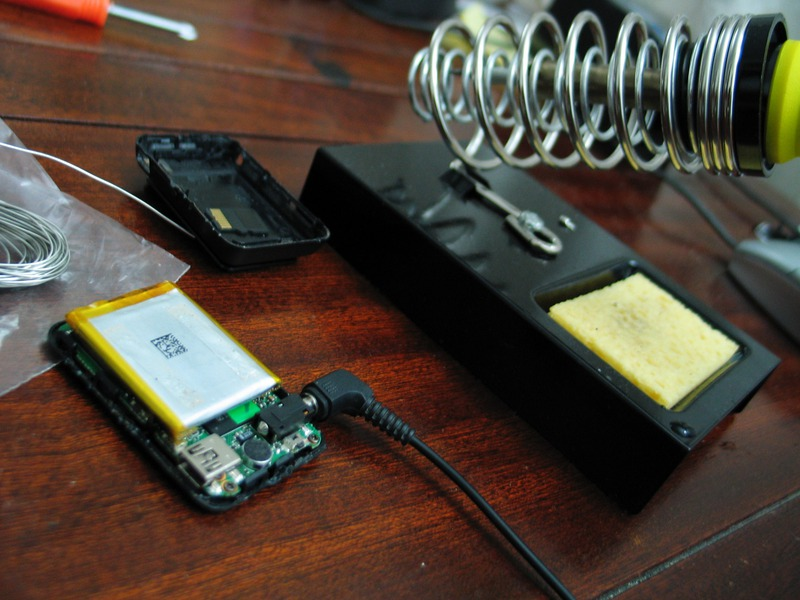
\includegraphics[width=\linewidth]{appendices/logistics/2011-06-30-22.44.32-Jarvist Frost-CanonG5-IMG_0083 - fixing Sansa Clip MP3 Player--orig.jpg}} 
 \caption{Fixing the Sansa Clip MP3 player. \pic{Jarvist Frost}}
 \label{sansa fix}
\end{marginfigure}

Music was provided by a Sansa Clip+ MP3 player wired into a pair of folding travel speakers.

The travel speakers could operate of 4 internal AAA batteries, but were found to be more powerful and longer lasting in the cold cave atmosphere when powered over USB wired directly into a battery pack of 4 AA Eneloop NiMh cells.

Similarly, the MP3 player was recharged from a 2xAA NiMh
---\textgreater{} USB `emergency phone charger', but was found to be happy to charge off the unregulated eneloop battery pack as well.*
  
In 2011 we moved entirely to just using the 4AA Eneloops + PP3 clip /   micro USB adapter to directly power both the speakers \& recharge the Sansas.

As well as music (of various tastes!) audio comedy has been a mainstay of underground camp, particularly in the evenings before falling asleep. \textit{Blackadder}, \textit{Father Ted}, \textit{Dead Ringers}, \textit{Little Britain}, \textit{League of Gentleman}, \textit{The Mighty Boosh} and \textit{The Ascent of Rum Doodle} have all proved popular over the years.


\section{Ambience}

Cheap tea-lights were taken down to camp and festooned on the cracked rock walls around the tent.

A couple of stubby `church' candles were also brought down (bought from `Tiger'), and were found to endure the cold atmosphere better than the tea lights (which tend to burn a hole through the core rather than burn all the wax).

This was reassuring, particularly for first time campers, and offered reassurance and sufficient light to go for a pee.

In 2011 we added `AA battery' powered white fairy lights. These were bought cheaply from dx.com, and were found to run (via resistor limiting) for an almost infinite time at a very low level, just enough to orientate oneself when waking at night. The most pleasant ones were `warm white' which had a very candle-flame like glow, even with mostly depleted batteries.

\section{Toiletry}

Excrement was deposited directly into compostable corn-starch bags, of the size used as standard compost bin caddy's and bought from a local Sainsburys. They were generally considered as `single use' -- except for when supplies ran rather low towards the end! These were then tied together, sealed in an additional non-biodegradable freezer bag and kept in a Daren drum.

Standard rolls of toilet paper were taken down, but kept in a resealable plastic bag to prevent damping in the cave atmosphere.

A alcohol based gel hand sanitiser was used for obvious reasons of hygiene.

Once suitably full, the Daren drum was portered out of the cave, and the biodegradable contents emptied into the latrine on the mountaintop.

\name{Jarvist Frost}
